\section{[WIP]Benutzerf"uhrung}

\subsection{Elemente der grafischen Benutzeroberfl"ache}

\begin{figure}[htb]
\centering
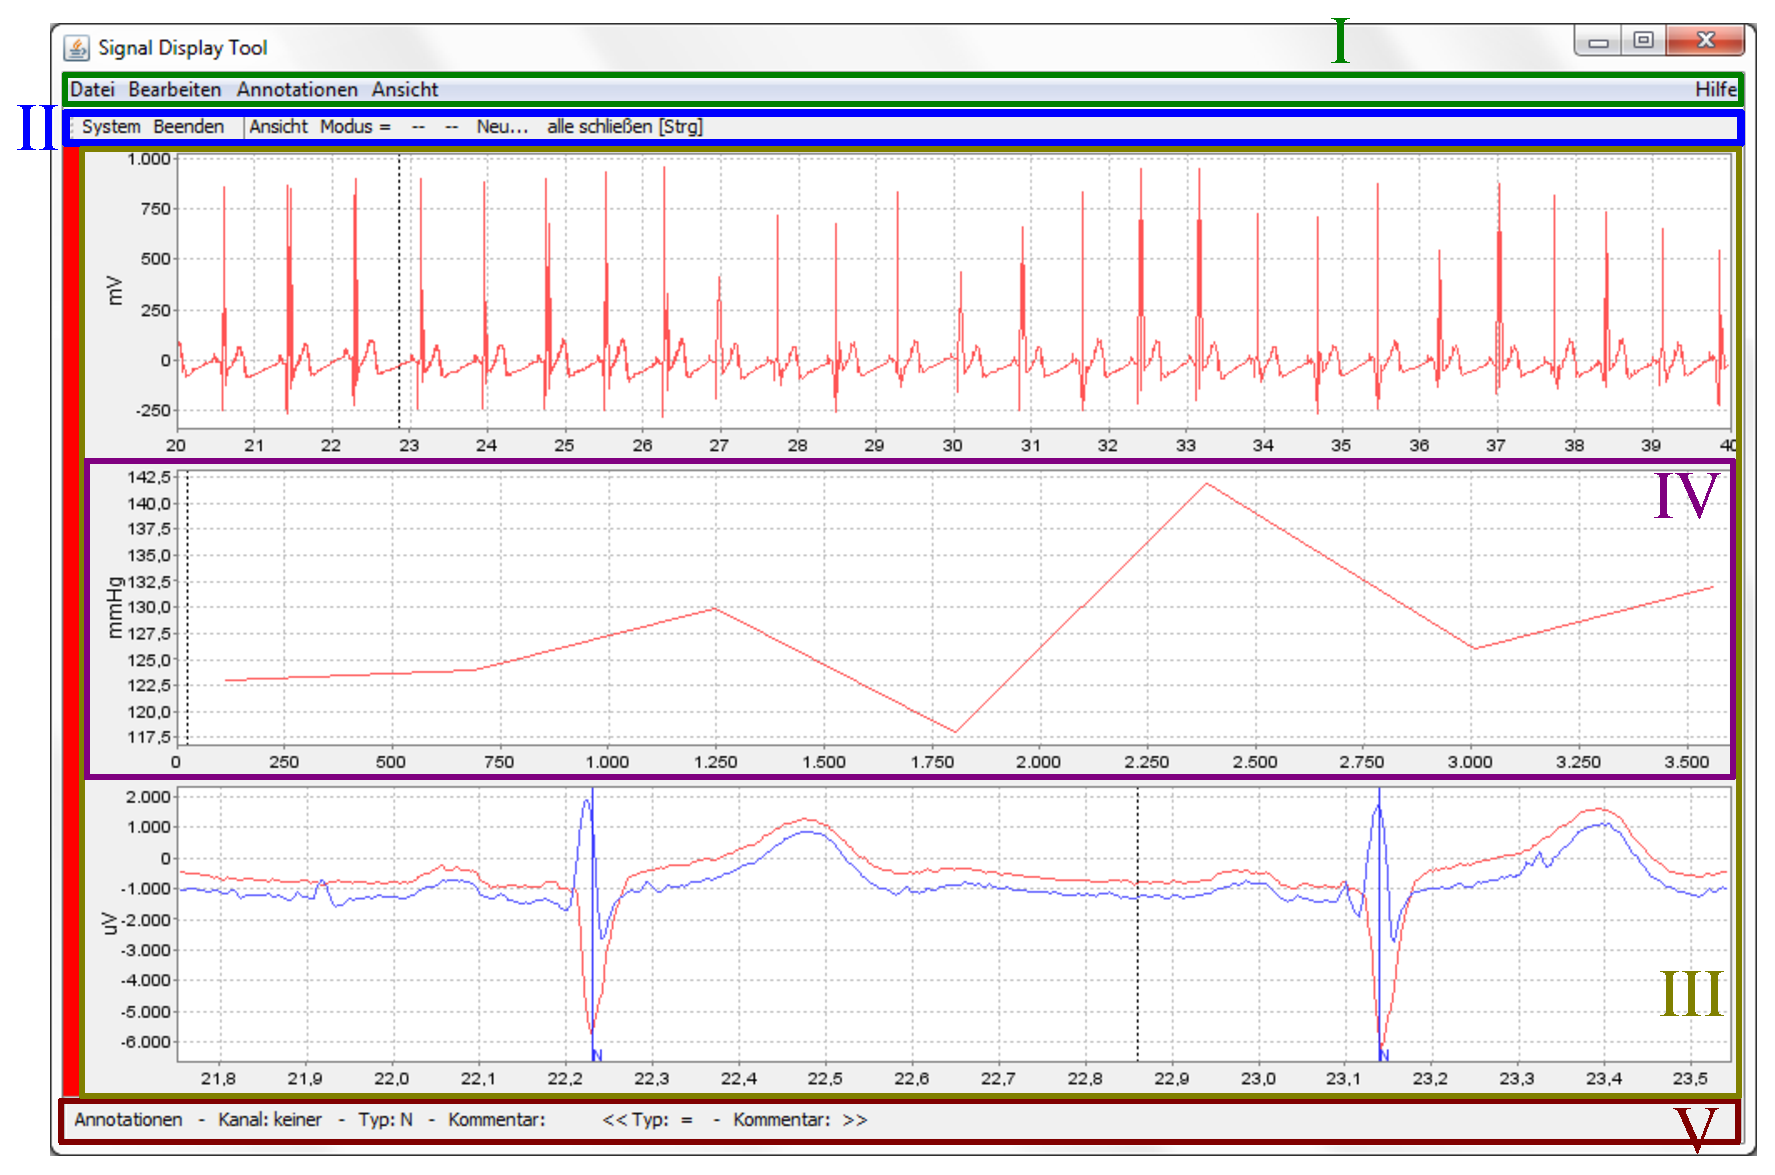
\includegraphics[width=\textwidth]{bilder/programm_ansicht.eps}
\caption[Klassen der grafischen Elemente]{Klassen der grafischen Elemente: I \texttt{Menus}, II \texttt{Toolbar}, III \texttt{SignalPanel}, IV \texttt{SignalView}, V \texttt{StatusBar}}
\label{pic:gui_elements_and_classes}
\end{figure}

In \picref{gui_elements_and_classes} sind die einzelnen Bestandteile der \ac{GUI} hervorgehoben.
Interaktionen zwischen dem Benutzer und dem Programm erfolgen "uber f"unf Hauptkomponenten:
\begin{itemize}
	\item Men"uzeile durch die Klasse \class{Menus} repr"asentiert
	\item Werkzeugleiste als Klasse \class{Toolbar}
	\item Statuszeile zum Anzeigen von Informationen mithilfe der Klasse \class{StatusBar}
	\item einzelne Diagramme als \class{SignalView}s zur Anzeige der Signalverl"aufe (im folgendem Signalansichten genannt)
	\item Zusammenfassung aller Signalansichten auf dem fl"achengr"o{\ss}tem Bestandteil, dem \class{SignalPanel}
\end{itemize}
W"ahrend das Men"u, die Werkzeugleiste und die Signalansichten Eingaben von dem Benutzer verarbeiten, dient die Statuszeile ausschlie{\ss}lich der Pr"asentation von Informationen.
Die grafische Darstellung der Klasse \class{SignalPanel} bleibt f"ur den Nutzer gr"o{\ss}tenteils verborgen, da es sich hierbei um ein organisatorisches Programmelement handelt (siehe dazu \secref{signalpanel_organisation}).

\begin{figure}[htb]
\centering
\includegraphics[angle=-90, width=0.9\textwidth]{bilder/package_ui_ubersicht.pdf}
\caption{"Ubersicht "uber das \class{ui}-Paket}
\label{pic:package_ui_ubersicht}
\end{figure}

Ein "Ubersicht die Klassenhierarchie ist in \picref{package_ui_ubersicht} dargestellt.
Bis auf die \class{SignalView}-Klasse sind alle grafischen Komponenten nach dem Singleton-Entwurfsmuster implementiert (vgl. \secref{singleton}).
Durch diese Entscheidung ist einerseits garantiert, dass die grafischen Elemente nur einmal in der Programminstanz vorkommen und au{\ss}erdem kann auf sie vereinfacht zugegriffen werden ("ahnlich globalen Variablen).

%- alle Elemente Singleton (bis auf \class{SignalView})

\subsection{[WIP]Visualisierung der Signalverl"aufe}

\subsubsection{Die genutzte \jfcNS-Bibliothek}

F"ur die Darstellung der Signalverl"aufe in Diagrammen wird die \javaNS-Bibliothek \jfc genutzt.
\jfc wird, ebenso wie das \usNS-Format, unter der \ac{lgpl} zur freien Nutzung angeboten.
Mithilfe der \jfcNS-Bibliothek k"onnen Diagramm unterschiedlicher Art zur Visualisierung von Daten dargestellt werden.
Neben der Vielzahl der unterst"utzten Diagrammtypen werden zus"atzlich die dynamische ver"anderbare Graphen unterst"utzt.
%Zudem sind durch umfangreiche Einstellm"oglichkeiten die Diagramme ausgesprochen individualisierbar.
Die umfangreichen Einstellm"oglichkeiten bei der Anpassung der Diagramme erm"oglichen eine nahezu nahtlose Integration der Bibliothekselemente in das bestehende grafischen Gesamtbild.
Zudem bietet die \jfcNS-Bibliothek, zus"atzlich zur grafischen Veranschaulichung von Daten, auch grafische Elemente um Bereiche oder bestimmte Punkte in einem Diagramm gesondert hervorheben zu k"onnen.

%- Nutzung von \jfc (\ac{lgpl})
%- langsam bei der darstellung vieler Datenpunkte

\subsubsection{Die Wrapper-Klasse \class{SignalView}}

F"ur die Integration der Diagramme in die \ac{GUI} als Signalansichten existiert die Klasse \class{SignalView}.
Objekte der Klasse haben die Aufgabe, die durch die \class{DataController} bereit gestellten Daten dem Benutzer grafisch zu veranschaulichen.
\class{SignalView} ist eine Unterklasse der Klasse \class{ChartPanel} aus \jfc und bildet somit das Verbindungselement zwischen dem Programm und der genutzten Bibliothek.
Ein \class{SignalView}-Objekt ist somit grafisch ein Diagramm auf der Benutzeroberfl"ache (vgl. mit \picref{gui_elements_and_classes}).
Die Darstellung der Daten erfolgt durch zwei Varianten.
Darstellung von kontinuierlich abgetasteten Signalen (\emph{Signals}) und Einzelwertezeitreihen (\emph{Values}) erfolgt als Liniendiagramm der Werte "uber der Zeit.
Die grafische Pr"asentation von Annotationen ist durch senkrechte Striche in den Diagrammen realisiert.

Um die Daten darzustellen muss der entsprechende \class{DataController} der Signalansicht hinzugef"ugt werden.
Es wird sichergestellt, dass jeder \class{DataController} nur genau einmal ein und demselben \class{SignalView}-Objekt hinzugef"ugt werden kann.
Jeder \class{SignalView} kann beliebig viele \class{DataController}-Objekte speichern und darstellen.
\class{SignalView} implementiert das Interface \class{DataChangeListener} des \code{data}-Paketes und ist daher in der Lage dynamisch auf "Anderungen von Daten zu reagieren.
Wird z.\,B. eine Annotation durch den Benutzer dem Datensatz hinzugef"ugt oder ver"andert, so wird in jeder Signalansicht diese "Anderung auch grafisch dargestellt (sofern der entsprechende Kanal dargestellt wird).

Neben der grafischen Darstellung der Daten bietet die \class{SignalView}-Klasse weitere optische R"uckmeldung f"ur den Nutzer.
So wird die aktuelle Mausposition innerhalb eines Diagramms, in Bezug auf die Zeitachse (Abszisse) durch eine gestrichelte senkrechte Linie hervorgehoben.
Die Hervorhebung erfolgt nicht nur in dem Diagramm, "uber dem der Mauszeiger sich gerade befindet, sondern in allen dargestellten Diagrammen.
Zudem wird die Signalansicht, "uber der sich der Mauszeiger befindet, visuell durch Ver"anderung der Hintergrundfarbe markiert.
Damit ist f"ur den Nutzer ersichtlich, welches Diagramm seine Eingaben empf"angt.
Die Verarbeitung der Maus- und Tastatureingabe des Nutzers durch zwei innere Klassen \class{Signal\-View\-Mouse\-Adapter} und \class{Signal\-View\-Key\-Adapter}.
Details zur Behandlung der Benutzereingabe sind im \secref{userinput} weiter unten er"ortert.

Das genutzte \jfcNS-Paket bietet die M"oglichkeit einem Diagramm eine Datenreihe mit mehreren Tausend Datenpunkten zuzuordnen.
Die Wahl des darzustellenden Ausschnitts kann durch den Benutzer durchgef"uhrt werden und wird durch die Bibliothek komplett unterst"utzt.
Die Zeit, die die Bibliothek ben"otigt um ein Diagramm mit all seinen Komponenten darzustellen, sinkt mit der Anzahl der Datenpunkte.
Obwohl von \jfc ein Renderer (das Objekt dass die Datenpunkte in dem Diagramm darstellt) f"ur viele Datenpunkte angeboten wird, sinkt die Darstellungsgeschwindigkeit bei \unit{3000} oder mehr Datenpunkten so stark, dass die Aktualisierung der Anzeige nicht mehr fl"ussig erscheint.
Das Programm ben"otigt zu viel Zeit um die Diagramme auf dem Bildschirm zu zeichnen, dass die Verarbeitung der Benutzereingabe und die Darstellung merklich verz"ogert erfolgen.
Dieses Problem wird in der eingereichten Implementierung umgangen, indem den Diagramm-Objekten eine begrenzte Anzahl an Datenpunkten "ubergeben wird.
Die Zahl der dargestellten Datenpunkte ist auf die Breite in Pixeln der Diagramme festgelegt.
Damit bleibt die Darstellung fl"ussig aber es entstehen visuelle Artefakte die durch das Downsampling bedingt sind.
Diese Darstellungsartefakte nehmen mit Erh"ohung der Zoomstufe ab, da umso mehr Datenpunkte dargestellt werden, je kleiner der Signalausschnitt wird (gr"o{\ss}ere Pixelaufl"osung pro Zeiteinheit).

%- Klasse \class{SignalView}
%- erh"alt Daten von \class{DataController} aus dem \code{data}-Paket
%- unterscheidet nur zwischen Annotationen und Daten
%- Markierung der Mausposition durch \emph{Crosshair} (gestrichelte Linie)
%- Hervorhebung der Signalansicht, die gerade Mausfokus hat
%- Einschr"ankung durch Begrenzung der Punkte auf die Pixelbreite des entsprechenden Diagramms

\subsubsection{Dynamische Reaktion auf Ver"anderung der Daten}



\subsection{[WIP]Gr"o{\ss}enbestimmung und Positionierung der Signalansichten durch \class{SignalPanel}}
\label{sec:signalpanel_organisation}

- organisationseinheit

\subsection{[WIP]Verarbeitung der Benutzereingabe im Paket \class{ui}}
\label{sec:userinput}


\subsubsection{[WIP]Koordiniertes Zoomen und Scrollen durch \class{SignalPanel}}

- Observer-Prinzip
- zwei eigene Managerklassen (Unabh"angigkeit) \class{ScrollLockManager}, \class{ZoomLockManager}

\subsubsection{[WIP]Verarbeitung der Benutzereingaben zur Steuerung der Ansicht}

- Einf"ugen und Entfernen von Datenkan"alen
- Steuerung der Ansicht "uber Zeitfenster
- Legende anzeigen
- \class{SignalView} stellt dar
- Datenzugriff "uber abstrakte Definition von \class{DataController}
- Subklassen verarbeiten Maus- und Tastatureingabe

\subsubsection{[WIP]Verarbeitung und Ver"anderung von Annotationen}

- Einf"ugen von Annotationen "uber \class{AnnotationManager}
- Dreiecksbeziehung von \class{Annotation\-Controller}, \class{AnnotationList} und \class{AnnotationManager} erl"autern
- Suchalgorithmus zum finden der aktuellen Annotation
- "Anderung wird durch die Implementierung vom Interface \class{Data\-Change\-Listener} automatisiert aktualisiert

% EOF
